% ============================================================
%  APCS 初級 Python 考前總複習
%  依據官方題本（程式識讀 30 題 + 程式實作 3 題）整理
%  編譯方式：xelatex apcs_review.tex（需安裝 ctex 套件）
% ============================================================
\documentclass[12pt, a4paper]{ctexart}

% ---------- 套件 ----------
\usepackage{geometry}
\usepackage{xcolor}
\usepackage{minted}
\usepackage[most, breakable]{tcolorbox}
\usepackage{enumitem}
\usepackage{booktabs}
\usepackage{amsmath}
\usepackage{amssymb}
\usepackage{tikz}
\usetikzlibrary{arrows.meta, positioning, shapes.geometric, fit, calc}
\usepackage{titlesec}
\usepackage{fancyhdr}
\usepackage{setspace}
\usepackage[hidelinks]{hyperref}
\usepackage[useregional=false, datesep={/}]{datetime2}

% ---------- 版面 ----------
\geometry{top=2.8cm, bottom=2.8cm, left=3.2cm, right=3.2cm, headheight=14pt}
\setstretch{1.15}

% ---------- Monospace 字型：Menlo（清晰，macOS 終端機預設）----------
\setmonofont{Menlo}[Scale=0.88]

% ---------- inline code：圓角底色框（tcolorbox on line）----------
\tcbuselibrary{skins}
\newtcbox{\ic}{on line,
  arc=2pt,
  boxsep=0pt, left=3pt, right=3pt, top=1.5pt, bottom=1.5pt,
  colback=inlinebg, colframe=inlinebg,
  fontupper=\ttfamily\small,
  nobeforeafter,
}
% 讓 \texttt 直接套用 inline code 樣式（排除特殊環境另處理）
\let\origtt\texttt
\renewcommand{\texttt}[1]{\ic{#1}}

% ---------- Latin 字型：Palatino（Zapf 設計，字寬寬敞，與宋體和諧）----------
\setmainfont{Palatino}[
  UprightFont    = {Palatino},
  BoldFont       = {Palatino Bold},
  ItalicFont     = {Palatino Italic},
  BoldItalicFont = {Palatino Bold Italic},
]

% ---------- 中文字型：粗體改用宋體粗體，不用黑體 ----------
\setCJKmainfont{Songti TC}[
  BoldFont   = {Songti TC Bold},
  ItalicFont = {Kaiti SC},
]

% ---------- 封面專用字型 ----------
\newfontfamily\coverlatin{Optima}
\newCJKfontfamily\covercjk{Hiragino Maru Gothic ProN}

% ---------- 主色 ----------
% ── Morandi 粉色系色票 ────────────────────────────────────────
% ink：字色，暖黑
\definecolor{ink}{RGB}{32, 28, 28}
% accent：主要強調色 — 莫蘭迪玫瑰灰紫，用於章節標題與分隔線
\definecolor{accent}{RGB}{140, 108, 118}
% muted：次要灰色（頁眉、行號等）
\definecolor{muted}{RGB}{130, 118, 115}
% codebg：程式碼區塊底色，極淡暖灰
\definecolor{codebg}{RGB}{246, 244, 242}
% notebg：筆記框底色，接近白的淡粉
\definecolor{notebg}{RGB}{251, 248, 249}
% notebar：筆記框左邊線 — 莫蘭迪霧藍綠，與粉色互補
\definecolor{notebar}{RGB}{85, 128, 128}

% ---------- 識讀題目環境 ----------
% qbg/qbar：識讀題目框 — 暖灰玫瑰
\definecolor{qbg}{RGB}{251, 249, 248}
\definecolor{qbar}{RGB}{148, 132, 130}
\NewTColorBox{qbox}{m}{
  enhanced, unbreakable,
  colback=qbg, colframe=qbar!50,
  toprule=0.4pt, bottomrule=0.4pt, leftrule=2.5pt, rightrule=0.4pt,
  left=10pt, right=10pt, top=6pt, bottom=6pt,
  before upper={\small\setstretch{1.1}},
  title={\small 題目 #1},
  attach boxed title to top left={yshift=-2pt, xshift=6pt},
  boxed title style={colback=qbar, colframe=qbar,
    fontupper=\small\color{white},
    left=5pt, right=5pt, top=1pt, bottom=1pt},
  coltitle=white,
}

% ---------- 習題環境（暖橙色，與筆記框區分）----------
% exercbg/exercbar：習題框 — 莫蘭迪粉玫瑰
\definecolor{exercbg}{RGB}{253, 247, 248}
\definecolor{exercbar}{RGB}{175, 120, 128}
\NewTColorBox{exercise}{O{練一練}}{
  enhanced, breakable,
  colback=exercbg, colframe=exercbar,
  leftrule=3pt, toprule=0.4pt, bottomrule=0.4pt, rightrule=0.4pt,
  left=9pt, right=9pt, top=5pt, bottom=5pt,
  fontupper=\small,
  title={#1},
  attach boxed title to top left={yshift=-2pt, xshift=6pt},
  boxed title style={colback=exercbar, colframe=exercbar,
    fontupper=\small\color{white},
    left=4pt, right=4pt, top=2pt, bottom=2pt},
  coltitle=white,
  before upper={\setstretch{1.15}},
}

% ---------- 偽碼背景色 ----------
% pseudobg：偽碼底色，淡奶油粉
\definecolor{pseudobg}{RGB}{253, 250, 246}

% inlinebg：inline code 底色，極淡灰粉
\definecolor{inlinebg}{RGB}{240, 236, 238}

% ---------- 統一注記框（左邊粗線，無彩色背景）----------
\newtcolorbox{note}[1][]{
  enhanced, breakable,
  colback=notebg,
  colframe=notebar,
  leftrule=3pt, toprule=0.4pt, bottomrule=0.4pt, rightrule=0.4pt,
  left=9pt, right=9pt, top=5pt, bottom=5pt,
  fontupper=\small,
  title={#1},
  attach boxed title to top left={yshift=-2pt, xshift=6pt},
  boxed title style={
    colback=notebar, colframe=notebar,
    fontupper=\small\color{white},
    left=4pt, right=4pt, top=2pt, bottom=2pt,
  },
  coltitle=white,
  before upper={\setstretch{1.1}},
}

% 為了向後相容，三個舊名稱都指向同一個 note 環境
\NewTColorBox{examtip}{O{考試提示}}{
  enhanced, breakable,
  colback=notebg, colframe=notebar,
  leftrule=3pt, toprule=0.4pt, bottomrule=0.4pt, rightrule=0.4pt,
  left=9pt, right=9pt, top=5pt, bottom=5pt,
  fontupper=\small,
  title={#1},
  attach boxed title to top left={yshift=-2pt, xshift=6pt},
  boxed title style={colback=notebar, colframe=notebar,
    fontupper=\small\color{white},
    left=4pt, right=4pt, top=2pt, bottom=2pt},
  coltitle=white,
  before upper={\setstretch{1.1}},
}
\NewTColorBox{examwarn}{O{常見錯誤}}{
  enhanced, breakable,
  colback=notebg, colframe=notebar,
  leftrule=3pt, toprule=0.4pt, bottomrule=0.4pt, rightrule=0.4pt,
  left=9pt, right=9pt, top=5pt, bottom=5pt,
  fontupper=\small,
  title={#1},
  attach boxed title to top left={yshift=-2pt, xshift=6pt},
  boxed title style={colback=notebar, colframe=notebar,
    fontupper=\small\color{white},
    left=4pt, right=4pt, top=2pt, bottom=2pt},
  coltitle=white,
  before upper={\setstretch{1.1}},
}
\NewTColorBox{keypoint}{O{核心觀念}}{
  enhanced, breakable,
  colback=notebg, colframe=notebar,
  leftrule=3pt, toprule=0.4pt, bottomrule=0.4pt, rightrule=0.4pt,
  left=9pt, right=9pt, top=5pt, bottom=5pt,
  fontupper=\small,
  title={#1},
  attach boxed title to top left={yshift=-2pt, xshift=6pt},
  boxed title style={colback=notebar, colframe=notebar,
    fontupper=\small\color{white},
    left=4pt, right=4pt, top=2pt, bottom=2pt},
  coltitle=white,
  before upper={\setstretch{1.1}},
}

% ---------- 題目原文框 ----------
\newtcolorbox{problem}[2]{
  enhanced, breakable,
  colback=white,
  colframe=accent!35,
  toprule=0.6pt, bottomrule=0.6pt, leftrule=0.6pt, rightrule=0.6pt,
  left=10pt, right=10pt, top=8pt, bottom=8pt,
  title={\large #1 \hfill \small\color{white!80!accent} #2},
  attach boxed title to top left={yshift=-0.5pt},
  boxed title style={
    colback=accent, colframe=accent,
    fontupper=\small\color{white},
    left=6pt, right=6pt, top=3pt, bottom=3pt,
    sharp corners,
  },
  coltitle=white,
  before upper={\setstretch{1.2}\small},
}

% ---------- 標題樣式：乾淨，只用粗細和間距 ----------
\titleformat{\section}
  {\Large\color{accent}}{\thesection}{0.8em}{}
  [\vspace{2pt}{\color{accent!50}\hrule height 0.5pt}\vspace{2pt}]

\titleformat{\subsection}
  {\large}{\thesubsection}{0.7em}{}

\titleformat{\subsubsection}[runin]
  {\normalsize\itshape}{\thesubsubsection}{0.5em}{}[\ ]

\titlespacing{\section}{0pt}{18pt}{8pt}
\titlespacing{\subsection}{0pt}{12pt}{4pt}

% ---------- 頁眉頁腳：極簡 ----------
\pagestyle{fancy}
\fancyhf{}
\fancyhead[L]{\small\color{muted} APCS 初級 Python 考前總複習}
\fancyhead[R]{\small\color{muted} \leftmark}
\fancyfoot[C]{\small\color{muted}\thepage}
\renewcommand{\headrulewidth}{0.3pt}
\renewcommand{\headrule}{\color{muted!50}\hrule width\headwidth height\headrulewidth}

% ---------- minted：真實 Python（彩色高亮 + 行號）----------
\setminted{
  style=xcode,
  bgcolor=codebg,
  fontsize=\small,
  linenos=true,
  numbersep=8pt,
  xleftmargin=4pt,
  breaklines=true,
  tabsize=4,
  baselinestretch=1.1,
}

% ---------- 偽碼環境（概念說明用，無行號，奶油底，text lexer）----------
\newminted[pseudocode]{text}{
  bgcolor=pseudobg,
  fontsize=\small,
  linenos=false,
  breaklines=true,
  tabsize=4,
  baselinestretch=1.1,
  xleftmargin=4pt,
}

% ---------- 版本號（手動維護）----------
\newcommand{\docversion}{v1.0}

% ============================================================
\begin{document}

% ===== 封面：文字排版，無色塊 =====
\begin{titlepage}
  \centering
  \vspace*{4cm}
  {\covercjk\coverlatin\fontsize{30}{38}\selectfont APCS 初級\\[0.5em] Python 考前總複習\par}
  \vspace{1.5cm}
  {\color{muted}\large 程式識讀 $\times$ 程式實作\par}
  \vspace{4cm}
  {\color{muted}\small
    \begin{tabular}{ll}
      程式識讀 & 30 題四選一，每題 5 分，共 150 分，75 分鐘 \\[4pt]
      程式實作 & 2 題，合計 100 分，75 分鐘 \\[4pt]
      核心能力 & 追蹤執行流程、條件／迴圈／遞迴、陣列操作 \\
    \end{tabular}
  \par}
  \vfill
  {\color{muted}\small 依據官方題本範例整理\par}
\end{titlepage}

\tableofcontents
\newpage

% ============================================================
\section{基礎語法速覽}
% ============================================================

\subsection{資料型別與運算子}

Python 常用型別：

\begin{center}
\begin{tabular}{llll}
\toprule
型別 & 範例 & 說明 & 轉換函式 \\
\midrule
\texttt{int} & \texttt{42, -5} & 整數 & \texttt{int(x)} \\
\texttt{float} & \texttt{3.14} & 浮點數 & \texttt{float(x)} \\
\texttt{str} & \texttt{'hello'} & 字串 & \texttt{str(x)} \\
\texttt{bool} & \texttt{True, False} & 布林值 & \texttt{bool(x)} \\
\texttt{list} & \texttt{[1, 2, 3]} & 可變序列 & \texttt{list(x)} \\
\bottomrule
\end{tabular}
\end{center}

\subsubsection*{算術運算子}

\begin{center}
\begin{tabular}{lll}
\toprule
運算子 & 說明 & 範例 \\
\midrule
\texttt{+, -, *, /} & 加減乘（浮點）除 & \texttt{7 / 2 = 3.5} \\
\texttt{//} & 整數除法（向下取整） & \texttt{7 // 2 = 3} \\
\texttt{\%} & 取餘數 & \texttt{7 \% 2 = 1} \\
\texttt{**} & 次方 & \texttt{2 ** 10 = 1024} \\
\bottomrule
\end{tabular}
\end{center}

\begin{examwarn}
  \texttt{//} 是\textit{向下取整}（floor），負數時要小心：
  \texttt{-7 // 2 = -4}，不是 \texttt{-3}。
  APCS 題目的 \texttt{(low + high) // 2} 在非負整數時沒問題。
\end{examwarn}

\subsection{輸入與輸出}

\begin{minted}{python}
n = int(input())                           # 讀一個整數
a, b = map(int, input().split())           # 同一行讀兩個整數
nums = list(map(int, input().split()))     # 讀一行多個整數成串列

print(a, b)             # 輸出，預設空格分隔，自動換行
print(a, b, sep='')     # 兩數緊鄰，無空格
print('Hi!', end='')    # 不換行
print(f'答案是 {a + b}')   # f-string 格式化
\end{minted}

\begin{examtip}
  實作題裡，\textit{輸出格式}是評分關鍵。看清楚是空格分隔還是換行，
  輸出 \texttt{None}（字串）還是沒有輸出，一個字都不能錯。
\end{examtip}

% ============================================================
\section{條件判斷}
\markboth{條件判斷}{}
% ============================================================

\subsection{if / elif / else 結構}

\begin{pseudocode}
if 條件A:
    # 執行 A
elif 條件B:
    # 執行 B（A 不成立才判斷）
else:
    # A、B 都不成立
\end{pseudocode}

\begin{keypoint}
  \textbf{if 與 elif 的根本差異}

  \texttt{if ... elif ...} 是一組，只執行第一個成立的分支，其餘全跳過。

  兩個獨立的 \texttt{if} 則各自判斷，兩個都可能執行。
\end{keypoint}

\subsection{條件順序錯誤（題目 17）}

題目問「評定等第的程式有幾個分數寫錯」：

\begin{minted}{python}
if s >= 90:
    print('A')
elif s >= 80:
    print('B')
elif s > 60:      # 錯：應寫 s >= 70 才能涵蓋 70~79
    print('D')    # 60~79 都跑進來印 D
elif s > 70:      # 這行永遠執行不到！
    print('C')
else:
    print('F')
\end{minted}

兩個 bug：\texttt{elif s > 60} 寫成 \texttt{>} 而非 \texttt{>=}，且順序放在 C 之前。
對照每個區間，看實際印出了什麼：

\begin{center}
\small
\begin{tabular}{p{2.2cm}ccl c}
\toprule
分數範圍 & 應印 & 實際印 & 原因 & 正確？ \\
\midrule
90\textasciitilde100 & A & A & — & $\checkmark$ \\
80\textasciitilde89  & B & B & — & $\checkmark$ \\
70\textasciitilde79  & C & D & \texttt{s > 60} 先攔截，印 D & \textbf{$\times$ ×10} \\
61\textasciitilde69  & D & D & \texttt{s > 60} 攔截，印 D & $\checkmark$ \\
60                   & D & F & \texttt{s > 60} 不含 60，落進 else & \textbf{$\times$ ×1} \\
0\textasciitilde59   & F & F & — & $\checkmark$ \\
\bottomrule
\end{tabular}
\end{center}

錯誤共 $10 + 1 = \mathbf{11}$ 個，答案 (B)。

\begin{examwarn}
  多層條件的地雷：
  \begin{enumerate}[label=\arabic*., itemsep=1pt, topsep=2pt, leftmargin=1.5em]
    \item 範圍是否有遺漏或重疊（\texttt{>} vs \texttt{>=}）
    \item 上面的 \texttt{elif} 先成立，下面的就不看
    \item 邊界值（如恰好等於臨界點的那個數）最容易出錯
  \end{enumerate}
\end{examwarn}

\subsection{獨立 if 的追蹤（題目 10）}

\begin{minted}{python}
count = 10
if count > 0:
    count = 11            # count = 11
if count > 10:            # 第二個獨立 if，仍會判斷
    count = 12
    if count % 3 == 4:    # 12 % 3 = 0，不等於 4
        count = 1
    else:
        count = 0         # count = 0
elif count > 11:          # 這個 elif 屬於第二個 if，被跳過
    count = 13
else:
    count = 14
if count:                 # count == 0 → False
    count = 15
else:
    count = 16            # count = 16
print(count)              # 輸出 16，答案 (D)
\end{minted}

\begin{exercise}[習題 — 條件追蹤]
  以下程式執行後，\texttt{x} 的值為何？
\begin{minted}{python}
x = 5
if x > 3:
    x = x + 2
if x > 6:
    x = x * 2
elif x > 4:
    x = x - 1
print(x)
\end{minted}
\end{exercise}

% ============================================================
\section{迴圈}
\markboth{迴圈}{}
% ============================================================

\subsection{for 迴圈與 range()}

\begin{minted}{python}
for i in range(5):           # i = 0, 1, 2, 3, 4
for i in range(2, 7):        # i = 2, 3, 4, 5, 6
for i in range(10, 0, -1):   # i = 10, 9, 8, ..., 1
for i in range(0, 101, 5):   # i = 0, 5, 10, ..., 100（共 21 個）
\end{minted}

\subsubsection*{range(1, 8, 2) 視覺化}

\begin{center}
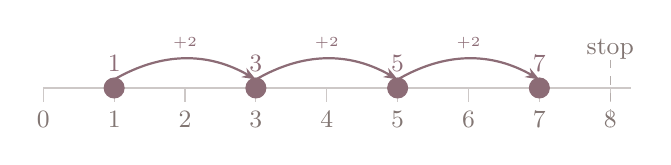
\begin{tikzpicture}[scale=0.9]
  \foreach \x in {0,...,8}{
    \draw[muted!40] (\x, 0) -- (\x, -0.2);
    \node[font=\small\color{muted}] at (\x, -0.45) {\x};
  }
  \draw[muted!40, -] (0,0) -- (8.3,0);
  \foreach \x in {1, 3, 5, 7}{
    \filldraw[accent] (\x, 0) circle (4pt);
    \node[font=\small\color{accent}] at (\x, 0.35) {\x};
  }
  \draw[accent, -{Stealth[length=5pt]}, thick] (1,0.12) to[bend left=30] node[above, font=\tiny]{+2} (3,0.12);
  \draw[accent, -{Stealth[length=5pt]}, thick] (3,0.12) to[bend left=30] node[above, font=\tiny]{+2} (5,0.12);
  \draw[accent, -{Stealth[length=5pt]}, thick] (5,0.12) to[bend left=30] node[above, font=\tiny]{+2} (7,0.12);
  \draw[muted!60, dashed] (8,0.4) -- (8,-0.55);
  \node[font=\small\color{muted}] at (8, 0.55) {stop};
\end{tikzpicture}
\end{center}

\begin{examtip}[題目 26：range 的元素數量]
  \texttt{range(0, 101, 5)} 含 21 個值（從 0 到 100），不是 20 個。

  公式：$\left\lfloor\dfrac{\text{stop} - \text{start} - 1}{\text{step}}\right\rfloor + 1$，或直接數 $0, 5, 10, \ldots, 100$。

  要印恰好 20 次，應改為 \texttt{range(0, 100, 5)} 或 \texttt{range(1, 101, 5)}。
\end{examtip}

\begin{exercise}[習題 — range 計算]
  不用電腦，直接算出以下 \texttt{range()} 各有幾個元素：
  \begin{enumerate}[label=(\alph*), itemsep=1pt, topsep=2pt]
    \item \texttt{range(3, 12)}
    \item \texttt{range(0, 20, 3)}
    \item \texttt{range(10, 1, -2)}
  \end{enumerate}
\end{exercise}

\subsection{while 迴圈}

\begin{minted}{python}
i = 0
while i < 10:
    print(i)
    i += 1       # 更新變數，確保能到達終止條件
\end{minted}

解「填空 while 條件」的策略：先確定迴圈\textit{應該在什麼情況停下}，
再把停止條件取反得到「繼續執行」的條件。

\begin{examtip}[題目 2：填入 while 條件]
  目標輸出：\texttt{[1][2][3][5][4][6]}

  外層 \texttt{for i in range(5)}，內層 \texttt{j} 從 0 開始，每次 \texttt{j = j + 2}，印出 \texttt{i + j}。

  \begin{itemize}[itemsep=1pt, topsep=2pt, leftmargin=1.5em]
    \item \texttt{i=0}：沒有 j 值滿足條件，不印
    \item \texttt{i=1}：\texttt{j=0} 印 \texttt{[1]}
    \item \texttt{i=2}：\texttt{j=0} 印 \texttt{[2]}，\texttt{j=2} 印 \texttt{[4]}（但輸出只有 \texttt{[2][3]}）
  \end{itemize}

  對照輸出，\texttt{i=2} 應只印一次，所以 \texttt{j < i}（即 \texttt{j < 2}）只允許 \texttt{j=0}。\\
  答案 (A)：條件為 \texttt{j < i}。
\end{examtip}

\subsection{巢狀迴圈與圖形（題目 5、19）}

解題步驟：
\begin{enumerate}[label=\arabic*., itemsep=0pt]
  \item 算每一列的空格數與符號數
  \item 外層 \texttt{i} 為列號，推出空格數和符號數關於 \texttt{i} 的公式
  \item 調整 \texttt{range()} 的 \texttt{start}、\texttt{stop}、\texttt{step}
\end{enumerate}

\textbf{題目 19}，要印出倒三角形（每列 \texttt{6-2i} 個星號）：

\begin{minted}{python}
# 目標輸出：
# * * * * * *    （i=0，6個星）
# * * * *        （i=1，4個星）
# * *            （i=2，2個星）
for i in range(3):
    for j in range(i):
        print(' ', end='')
    for k in range(6-2*i, 0, -1):   # 第二個參數填 0，答案 (C)
        print('*', end='')
    print('')
\end{minted}

\subsection{二維陣列巢狀迴圈（題目 18）}

計算 5×5 迷宮中，內部 3×3 格每格的四方向鄰居中值為 1 的總數：

\begin{minted}{python}
maze = [[1,1,1,1,1],
        [1,0,1,0,1],
        [1,1,0,0,1],
        [1,0,0,1,1],
        [1,1,1,1,1]]
count = 0
for i in range(1, 4):           # 內部 row
    for j in range(1, 4):       # 內部 col
        dir = [[-1,0],[0,1],[1,0],[0,-1]]   # 上右下左
        for d in range(4):
            if maze[i+dir[d][0]][j+dir[d][1]] == 1:
                count += 1
print(count)    # 答案 20，選 (B)
\end{minted}

% ============================================================
\section{函式與遞迴}
\markboth{函式與遞迴}{}
% ============================================================

\subsection{函式基本概念}

\begin{minted}{python}
def add(a, b):
    return a + b        # 遇到 return 立刻結束函式

result = add(3, 5)      # result = 8
\end{minted}

\begin{keypoint}
  函式執行到 \texttt{return} 就結束，\textit{後面的程式碼不會執行}。

  若函式沒有 \texttt{return}，或 \texttt{return} 後面沒有值，回傳 \texttt{None}。
\end{keypoint}

\subsection{遞迴的兩個必要條件}

\begin{enumerate}[label=\arabic*., itemsep=2pt]
  \item \textbf{終止條件（base case）}：讓遞迴能停下來的判斷
  \item \textbf{縮減問題規模}：每次呼叫必須讓問題往終止條件靠近
\end{enumerate}

\begin{minted}{python}
def factorial(n):
    if n <= 1:                    # 終止條件
        return 1
    return n * factorial(n - 1)  # 縮減：n 每次減 1

# factorial(5) = 5*4*3*2*1 = 120
\end{minted}

\textbf{題目 11}：計算 n 階乘的函式有 bug，
把第 3 行 \texttt{if n >= 0} 改為 \texttt{if n > 0} 即可正確終止，答案 (B)。

\subsubsection*{factorial(4) 呼叫展開樹}

\begin{center}
\begin{tikzpicture}[
  node distance=0.9cm and 1.6cm,
  nd/.style={draw=accent!50, rounded corners=3pt, fill=codebg,
             font=\ttfamily\small, inner sep=4pt, minimum width=2.8cm},
  ret/.style={font=\small\color{muted}, inner sep=2pt},
  arr/.style={-{Stealth[length=5pt]}, accent!60},
  rarr/.style={-{Stealth[length=5pt]}, accent!30, dashed},
]
  \node[nd] (f4) {factorial(4)};
  \node[nd, below=of f4] (f3) {factorial(3)};
  \node[nd, below=of f3] (f2) {factorial(2)};
  \node[nd, below=of f2] (f1) {factorial(1)};
  \node[ret, right=1.8cm of f1] (r1) {return \textbf{1}};
  \node[ret, right=1.8cm of f2] (r2) {return 2 × 1 = \textbf{2}};
  \node[ret, right=1.8cm of f3] (r3) {return 3 × 2 = \textbf{6}};
  \node[ret, right=1.8cm of f4] (r4) {return 4 × 6 = \textbf{24}};

  \draw[arr] (f4) -- node[left, font=\tiny\color{muted}]{呼叫} (f3);
  \draw[arr] (f3) -- (f2);
  \draw[arr] (f2) -- (f1);
  \draw[rarr] (f1) -- (r1);
  \draw[rarr] (f2) -- (r2);
  \draw[rarr] (f3) -- (r3);
  \draw[rarr] (f4) -- (r4);
\end{tikzpicture}
\end{center}

\begin{exercise}[習題 — 遞迴追蹤]
  給定以下函式，請問 \texttt{f(5)} 的回傳值為何？寫出展開過程。
\begin{minted}{python}
def f(n):
    if n <= 0:
        return 0
    return n + f(n - 2)
\end{minted}
\end{exercise}

\subsection{遞迴追蹤的方法}

\begin{enumerate}[label=\arabic*., itemsep=2pt]
  \item 先找\textit{終止條件}，知道哪些輸入直接回傳
  \item 從最小的 case 往上推，建立一張展開表
  \item 注意回傳後是否還有計算（\texttt{return f(n-1) + n} 中，\texttt{f(n-1)} 先算，回來才加 \texttt{n}）
\end{enumerate}

\textbf{題目 1}：\texttt{f(10)} 展開

\begin{minted}{python}
def f(i):
    if i > 0:
        if (i // 2) % 2 == 0:
            return f(i-2) * i
        return f(i-2) * (-i)
    else:
        return 1
\end{minted}

\begin{center}
\small
\begin{tabular}{@{} l p{4.8cm} p{3.6cm} r @{}}
\toprule
呼叫 & 條件（\texttt{(i//2)\%2}） & 計算式 & 回傳值 \\
\midrule
\texttt{f(0)}  & \texttt{i <= 0}，終止條件          & —                     & $1$ \\
\texttt{f(2)}  & $1\%2 = 1 \neq 0$，乘 $(-i)$      & $f(0)\times(-2)$      & $-2$ \\
\texttt{f(4)}  & $2\%2 = 0$，乘 $i$                 & $f(2)\times 4$        & $-8$ \\
\texttt{f(6)}  & $3\%2 = 1 \neq 0$，乘 $(-i)$      & $f(4)\times(-6)$      & $48$ \\
\texttt{f(8)}  & $4\%2 = 0$，乘 $i$                 & $f(6)\times 8$        & $384$ \\
\texttt{f(10)} & $5\%2 = 1 \neq 0$，乘 $(-i)$      & $f(8)\times(-10)$     & $\mathbf{-3840}$ \\
\bottomrule
\end{tabular}
\end{center}

\subsection{費式數列（題目 7、14）}

\begin{minted}{python}
# 遞迴版
def fib(n):
    if n < 2:
        return n
    return fib(n-1) + fib(n-2)

# 迴圈版（題目 7 的結構）
a, b = 0, 1
for i in range(2, N+1):
    temp = b
    b = a + b    # (a) 填 b = a+b
    a = temp
print(a)         # (b) 填 a
\end{minted}

\begin{examtip}
  迴圈版費式數列中，\texttt{temp = b} 的作用是\textit{暫存舊的 b 值}，避免 \texttt{b} 更新後再去算 \texttt{a = temp} 時拿到錯誤的值。

  用 Python 同時賦值可簡化為 \texttt{a, b = b, a + b}。
\end{examtip}

\textbf{題目 14}：\texttt{Mystery(9) = 34}，終止條件為 \texttt{x <= 1}，
推出 else 的算式是 \texttt{Mystery(x-2) + Mystery(x-1)}，答案 (D)。

\subsection{GCD 輾轉除法（題目 9、23）}

\begin{keypoint}
  \textit{輾轉除法原理}：$\gcd(a, b) = \gcd(b,\ a \bmod b)$

  每次把「余數」替換「較大數」，直到余數為 0，此時「較小數」就是 GCD。
\end{keypoint}

\begin{minted}{python}
# 迴圈版（題目 9：填入 while 迴圈內容）
i, j = 76, 48
while (i % j) != 0:
    k = i % j       # 保存余數
    i = j
    j = k           # (A) 正確答案
print(j)            # 印出 GCD = 4

# 遞迴版（題目 23：填入兩個 return）
def GCD(a, b):
    r = a % b
    if r == 0:
        return b          # 填 b
    return GCD(b, r)      # 填 GCD(b, r)，答案 (B)
\end{minted}

\subsection{互相遞迴（題目 8、13）}

兩函式互相呼叫時，追蹤時要記錄\textit{每次呼叫後要回來做什麼}（類似堆疊）。

\begin{minted}{python}
def f1(m):
    if m > 3:
        print(m); return
    else:
        print(m)
        f2(m + 2)
        print(m)       # f2 回來後才執行這行

def f2(n):
    if n > 3:
        print(n); return
    else:
        print(n)
        f1(n - 1)
        print(n)

f1(1)
# 執行順序：
#   f1(1) -> 印1 -> f2(3) -> 印3 -> f1(2) -> 印2
#         -> f2(4) -> 印4 -> 回 -> 印2
#         -> 回f2(3) -> 印3 -> 回f1(1) -> 印1
# 輸出：1 3 2 4 2 3 1
\end{minted}

題目 8 問「以下敘述何者為錯」。追蹤呼叫路徑：

\begin{itemize}[itemsep=1pt, topsep=3pt, leftmargin=1.5em]
  \item f1(1) 呼叫 f2(3)，f2(3) 呼叫 f1(2)，f1(2) 呼叫 f2(4)
  \item f2 被呼叫的位置：f2(3)、f2(4)，共 \textit{2 次}
\end{itemize}

選項 (C)「f2 一共被呼叫三次」是錯誤的，答案 (C)。

\subsection{遞迴冪次（題目 21）}

\begin{minted}{python}
def G(a, x):
    if x == 0:
        return 1
    else:
        return a * G(a, x - 1)

# G(a, x) = a^x
# G(3, 7) = 3^7 = 2187，答案 (B)
\end{minted}

% ============================================================
\section{串列（List）}
\markboth{串列（List）}{}
% ============================================================

\subsection{基本操作}

\begin{minted}{python}
a = [1, 3, 5, 7, 9]
print(a[0])          # 1（索引從 0 開始）
print(a[-1])         # 9（負索引從末尾算）
print(len(a))        # 5

a.append(11)         # 末尾加入
a.sort()             # 原地排序（升序）
b = sorted(a, reverse=True, key=lambda x: x)   # 回傳新串列
\end{minted}

\subsubsection*{串列索引示意}

\begin{center}
\begin{tikzpicture}[
  cell/.style={draw=accent!50, minimum width=1.2cm, minimum height=0.7cm,
               fill=codebg, font=\ttfamily\small},
  idx/.style={font=\small\color{muted}},
]
  \foreach \val/\i in {1/0, 3/1, 5/2, 7/3, 9/4}{
    \node[cell] (c\i) at (\i*1.3, 0) {\val};
    \node[idx] at (\i*1.3,  0.65) {\i};
    \pgfmathtruncatemacro{\neg}{\i - 5}
    \node[idx] at (\i*1.3, -0.65) {\neg};
  }
  \node[idx, anchor=east] at (-0.4,  0.65) {正索引};
  \node[idx, anchor=east] at (-0.4, -0.65) {負索引};
  \draw[accent!40, dashed] (-0.15, 0.38) -- (5.45, 0.38);
  \draw[accent!40, dashed] (-0.15,-0.38) -- (5.45,-0.38);
\end{tikzpicture}
\end{center}

\begin{exercise}[習題 — 串列索引]
  \texttt{a = [10, 20, 30, 40, 50]}，請問以下各式的值為何？
  \begin{enumerate}[label=(\alph*), itemsep=1pt, topsep=2pt]
    \item \texttt{a[2]}
    \item \texttt{a[-1]}
    \item \texttt{a[-3]}
    \item \texttt{len(a) - 1}（最後一個元素的正索引）
  \end{enumerate}
\end{exercise}

\subsection{串列初始化}

\begin{minted}{python}
a = [0] * 10                    # [0, 0, ..., 0]（10 個 0）
b = [i for i in range(101)]     # [0, 1, 2, ..., 100]  ← list comprehension
c = [i**2 for i in range(5)]    # [0, 1, 4, 9, 16]
\end{minted}

\begin{examtip}[題目 30：前綴和]
  \texttt{b = [i for i in range(101)]} 即 \texttt{b[i] = i}。

  接著 \texttt{a[i] = b[i] + a[i-1] = i + a[i-1]}，\texttt{a} 就是從 1 加到 \texttt{i} 的前綴和。

  \texttt{a[50] - a[30] = (1+\ldots+50) - (1+\ldots+30) = 31+32+\ldots+50 = 810}，答案 (D)。
\end{examtip}

\subsection{同時賦值（題目 15）}

Python 的同時賦值會先把右側全部算出來，再一次性賦值：

\begin{minted}{python}
a, b = b, a          # 交換兩個變數，不需要 temp

# 題目 15：
a = [1, 3, 5, 7, 9, 8, 6, 4, 2]
n = 9
for i in range(n):
    a[i], a[n-i-1] = a[n-i-1], a[i]   # 同時交換，反轉陣列
# 反轉後：[2, 4, 6, 8, 9, 7, 5, 3, 1]
# 但每個 i 都做，i=0 時換 a[0]↔a[8]，i=4 時換 a[4]↔a[4]……
# 最終 a = [1, 2, 3, 4, 5, 6, 7, 8, 9, 9]（含重複邊界）
# 印出第一個 n//2+1 = 5 對 → 1 2 3 4 5 6 7 8 9 9，答案 (C)
\end{minted}

\subsection{索引偏移（題目 25）}

\begin{minted}{python}
X = [0] * 10
for i in range(10):
    X[(i+2) % 10] = int(input())   # 輸入 0,1,...,9

# i=0 → X[2]=0；i=1 → X[3]=1；...；i=7 → X[9]=7
# i=8 → X[0]=8；i=9 → X[1]=9
# 結果：X = [8, 9, 0, 1, 2, 3, 4, 5, 6, 7]，答案 (D)
\end{minted}

\subsection{搜尋演算法（題目 6、22、29）}

\subsubsection*{線性搜尋}

\begin{minted}{python}
def linear_search(a, value):
    for i in range(len(a)):        # 逐一比較
        if a[i] == value:
            return i
    return -1
\end{minted}

100 個元素，找 \texttt{a[33]=100}：迴圈執行到 \texttt{i=33} 時找到，\texttt{while} 主體共執行 34 次（n1 = 34）。

\subsubsection*{二分搜尋}

\begin{minted}{python}
def binary_search(a, value):
    low, high = 0, len(a) - 1
    while low <= high:
        mid = (low + high) // 2
        if a[mid] == value:
            return mid
        elif a[mid] < value:
            low = mid + 1
        else:
            high = mid - 1
    return -1
\end{minted}

\begin{keypoint}
  二分搜尋每次縮減一半，100 個元素最多需 $\lceil\log_2 100\rceil = 7$ 次，
  本題實際追蹤為 5 次（n2 = 5）。\textit{前提：陣列必須已排序。}
\end{keypoint}

\textbf{題目 22}（二分搜尋有 bug）：函式目的是找「A 中大於 x 的最小值」。
當 \texttt{x=16}（已超出 A 最大值 14），\texttt{high} 最終指向 index 7，
\texttt{A[7]=14} 並非大於 16，程式回傳錯誤，答案 (D)。

\subsection{最大值、最小值追蹤（題目 24、29）}

\begin{minted}{python}
p = q = A[0]          # 同時初始化為第一個元素
for i in range(1, n):
    if A[i] > p:
        p = A[i]      # p 追最大值
    if A[i] < q:
        q = A[i]      # q 追最小值
\end{minted}

\begin{examwarn}[題目 24：「不一定正確」的陷阱]
  若陣列所有元素相同，則 \texttt{p == q}，「\texttt{q < p}」為 False。

  選項 (C) \texttt{q < p} 不一定正確，為答案。
\end{examwarn}

\textbf{題目 29}：程式初始 \texttt{M = N = s = -1, 101, 3}，
只有 3 個元素，\texttt{elif A[i] < N} 用 \texttt{elif} 而非 \texttt{if}，
當 \texttt{A[i] > M} 成立時跳過最小值判斷，找測資讓 \texttt{A[0] < A[1] < A[2]}
才能觸發錯誤，答案 \texttt{[80, 90, 100]}，選 (B)。

% ============================================================
\section{程式識讀技巧}
\markboth{程式識讀技巧}{}
% ============================================================

\subsection{執行流程追蹤四步驟}

\begin{enumerate}[label=\arabic*., itemsep=3pt]
  \item \textbf{找起點}：從 top-level 程式或函式呼叫點開始
  \item \textbf{建變數表}：每個變數一欄，逐行更新
  \item \textbf{展開迴圈/遞迴}：把每輪的值逐一記錄，不要跳步
  \item \textbf{確認輸出時機}：\texttt{print} 在迴圈裡還是外？遞迴回來後還有沒有輸出？
\end{enumerate}

\subsection{死程式碼（Dead Code，題目 27）}

「永遠執行不到」的程式碼：

\begin{minted}{python}
def F(a):
    while a < 10:
        a = a + 5
    # while 結束後：a 只可能是 10（0+5+5）或 15、20...
    if a < 12:
        a = a + 2    # 若 a=10 → a 變 12
    if a < 11:
        a = 5        # a 只可能是 12, 15, 20...，永遠 >= 11，這行執行不到
\end{minted}

答案 (C)：\texttt{a = 5} 永遠不會執行。

\subsection{冗餘程式碼（題目 20）}

「冗餘」= 移除後程式行為不變。\\
判斷策略：某段程式計算的值，在後面\textit{馬上就被覆蓋或根本不用}。

\texttt{Change \% 1} 的結果永遠是 0（任何整數除以 1 餘 0），
D 區的 \texttt{Change = Change \% 1} 把 Change 清零，
但清完之後已經沒有後續使用，而 D 區的 \texttt{print} 只印出「1 元硬幣」的張數，
\texttt{Change = Change \% 1} 這行是冗餘的，答案 (D)。

\subsection{填空題策略（題目 2、3、9、12、16、19、23）}

\begin{enumerate}[label=\arabic*., itemsep=3pt]
  \item \textbf{逆向推導}：已知輸出，從輸出往回推條件或算式
  \item \textbf{代入選項}：把四個選項逐一代入，看哪個產生正確結果
  \item \textbf{邊界驗證}：除了正常情況，也試試最小值或最大值
\end{enumerate}

% ============================================================
\section{程式實作題攻略}
\markboth{程式實作題攻略}{}
% ============================================================

\subsection{解題流程}

\begin{enumerate}[label=\arabic*., itemsep=3pt]
  \item \textbf{讀清楚輸入格式}：幾行？每行幾個數？用什麼隔開？
  \item \textbf{讀清楚輸出格式}：空格？換行？特殊情況（如 \texttt{None}）？
  \item \textbf{先對範例}：用題目的範例輸入手動跑一遍，確認理解題意
  \item \textbf{實作並測試}：先過範例，再想邊界情況
\end{enumerate}

\subsection{實作題型一：七言對聯（2021/9）}

\begin{problem}{七言對聯}{程式實作 2021 年 9 月}
\textbf{問題描述}

每首七言對聯有兩句，每句七個字，每字的平仄以 0（平聲）或 1（仄聲）表示。
請檢查對聯是否符合以下三條規則，並輸出所有違反的規則編號：

\begin{itemize}[itemsep=1pt, topsep=2pt]
  \item \textbf{規則 A（二四不同二六同）}：每句第 2 字與第 4 字的平仄必須不同；第 2 字與第 6 字的平仄必須相同。（兩句都要檢查）
  \item \textbf{規則 B（仄起平收）}：第一句第 7 字必須是仄聲，第二句第 7 字必須是平聲。
  \item \textbf{規則 C（同聯相對）}：第一句的第 2、4、6 字的平仄，必須分別與第二句的第 2、4、6 字的平仄相反。
\end{itemize}

\medskip
\textbf{輸入格式}

第一行為正整數 $n$（$1 \le n \le 30$），表示有幾首對聯。
接下來每 2 行為一首對聯，每行 7 個數字（0 或 1），以空白間隔。

\textbf{輸出格式}

輸出 $n$ 行。每行列出該對聯違反的規則字母（依字母順序，無空白）。若全部符合則輸出 \texttt{None}。

\medskip
\textbf{範例}

\begin{center}
\begin{tabular}{p{4cm} p{4cm}}
\small\textbf{輸入} & \small\textbf{輸出} \\[2pt]
\ttfamily\small
1 \newline
1 0 0 0 0 1 1 \newline
0 1 0 0 1 1 0
&
\ttfamily\small AC
\end{tabular}
\end{center}
\end{problem}

\medskip
知識點：陣列索引比對、多條件判斷、集合去重、排序輸出

\begin{minted}{python}
n = int(input())
for _ in range(n):
    r1 = list(map(int, input().split()))
    r2 = list(map(int, input().split()))
    bad = set()

    # 規則 A：二四不同二六同（索引 1,3,5，從 0 開始）
    if r1[1] == r1[3] or r1[1] != r1[5]:
        bad.add('A')
    if r2[1] == r2[3] or r2[1] != r2[5]:
        bad.add('A')

    # 規則 B：仄起平收（第7字 = 索引6；仄=1，平=0）
    if r1[6] != 1 or r2[6] != 0:
        bad.add('B')

    # 規則 C：同聯相對（第2,4,6字，索引1,3,5 必須互反）
    for idx in [1, 3, 5]:
        if r1[idx] == r2[idx]:
            bad.add('C')

    print(''.join(sorted(bad)) if bad else 'None')
\end{minted}

\subsection{實作題型二：裝飲料（2024/10）}

\begin{problem}{裝飲料}{程式實作 2024 年 10 月}
\textbf{問題描述}

一個冷飲杯的內層空間由上下兩個長方體相接組成：
下方底面為 $w_1 \times w_1$ cm²，高 $h_1$ cm；上方底面為 $w_2 \times w_2$ cm²，高 $h_2$ cm（$w_1 < w_2$）。

已知依序倒入 $N$ 杯冰水，體積分別為 $V_1, V_2, \ldots, V_N$（單位 ml，$1\text{ cm}^3 = 1\text{ ml}$）。
求每次加水後水位上升高度的\textbf{最大值}。杯子裝滿後水位不再上升（上升值為 0）。
每次上升高度保證為整數。

\medskip
\textbf{輸入格式}

第一行正整數 $N$（$1 \le N \le 10$）。第二行四個正整數 $w_1,w_2,h_1,h_2$（$1 \le w_1 < w_2,\ h_1,h_2 \le 50$）。
第三行 $N$ 個正整數，每次加水體積不超過 $10^6$。

\textbf{輸出格式}

一個整數，為水位上升高度的最大值。

\medskip
\textbf{範例}

\begin{center}
\begin{tabular}{p{4cm} p{4cm}}
\small\textbf{輸入} & \small\textbf{輸出} \\[2pt]
\ttfamily\small
2 \newline
5 10 12 8 \newline
400 600
&
\ttfamily\small 13
\end{tabular}
\end{center}

說明：第一杯 400 ml 裝入後水升 13 cm，第二杯 600 ml 裝入後水升 6 cm，最大值為 13。
\end{problem}

\medskip
知識點：分段體積計算（下段/上段）、加水後高度、最大值追蹤

\begin{minted}{python}
N = int(input())
w1, w2, h1, h2 = map(int, input().split())
vols = list(map(int, input().split()))

cap1 = w1 * w1 * h1       # 下段總容量
cap2 = w2 * w2 * h2       # 上段總容量

cur_h = 0
max_rise = 0

for v in vols:
    # 計算目前水量
    if cur_h <= h1:
        cur_v = cur_h * w1 * w1
    else:
        cur_v = cap1 + (cur_h - h1) * w2 * w2

    new_v = min(cur_v + v, cap1 + cap2)  # 不超過總容量

    # 計算新高度
    if new_v <= cap1:
        new_h = new_v // (w1 * w1)
    else:
        new_h = h1 + (new_v - cap1) // (w2 * w2)

    rise = new_h - cur_h
    max_rise = max(max_rise, rise)
    cur_h = new_h

print(max_rise)
\end{minted}

\subsection{實作題型三：遊戲選角（2024/1）}

\begin{problem}{遊戲選角}{程式實作 2024 年 1 月}
\textbf{問題描述}

遊戲中每個角色有攻擊力和防禦力兩個屬性，綜合能力定義為：
\[
  \text{綜合能力} = \text{攻擊力}^2 + \text{防禦力}^2
\]
給定 $n$ 名角色的屬性，找出\textbf{綜合能力第二高}的角色，輸出其攻擊力與防禦力。
題目保證所有角色的綜合能力皆相異。

\medskip
\textbf{輸入格式}

第一行整數 $n$（$3 \le n \le 20$）。接下來 $n$ 行，每行兩個整數，分別為攻擊力和防禦力（$1 \le$ 各值 $\le 100$）。

\textbf{輸出格式}

一行，兩個整數，依序為綜合能力第二高角色的攻擊力與防禦力，以空白間隔。

\medskip
\textbf{範例}

\begin{center}
\begin{tabular}{p{3.5cm} p{4.5cm}}
\small\textbf{輸入} & \small\textbf{輸出} \\[2pt]
\ttfamily\small
3 \newline
3 2 \newline
5 2 \newline
1 4
&
\ttfamily\small 1 4
\end{tabular}
\end{center}

說明：三名角色的綜合能力分別為 13、29、17，第二高（17）為第三位角色，輸出 1 4。
\end{problem}

\medskip
知識點：自定義排序 key（\texttt{lambda}）、找第二高值

\begin{minted}{python}
n = int(input())
chars = []
for _ in range(n):
    a, d = map(int, input().split())
    chars.append((a, d, a**2 + d**2))

# 依綜合能力降序排列
chars.sort(key=lambda x: x[2], reverse=True)

# 題目保證所有角色綜合能力相異，第二高即 index = 1
print(chars[1][0], chars[1][1])
\end{minted}

\begin{examtip}
  \begin{itemize}[itemsep=1pt, topsep=0pt, leftmargin=1.5em]
    \item \texttt{sorted()} 回傳新串列，原串列不變
    \item \texttt{list.sort()} 原地排序，回傳 \texttt{None}
    \item 兩者都可接受 \texttt{key=} 和 \texttt{reverse=True}
  \end{itemize}
\end{examtip}

% ============================================================
\newpage
\section{程式識讀 完整題庫}
\markboth{程式識讀 完整題庫}{}
% ============================================================

% ============================================================
%  程式識讀 完整題庫（30 題）
%  依據《程式識讀題目範例 Python 題本》原文整理
% ============================================================

% 知識點標籤
\newcommand{\qskill}[1]{%
  \par\vspace{2pt}
  {\small\color{notebar}\textit{知識點：#1}}%
  \vspace{2pt}%
}

% 四個選項：每個都獨立一行，間距緊湊
\newcommand{\qchoices}[4]{%
  \vspace{3pt}
  \begin{enumerate}[label=(\Alph*), itemsep=1pt, topsep=1pt,
                    leftmargin=2.2em, parsep=0pt]
    \item #1
    \item #2
    \item #3
    \item #4
  \end{enumerate}
}

% -------- 題目 1 --------
\begin{qbox}{1}
給定右側函式 \texttt{f()}，當執行 \texttt{f(10)} 時，最終回傳結果為何？

\begin{minted}{python}
def f(i):
    if i > 0:
        if (i // 2) % 2 == 0:
            return f(i - 2) * i
        return f(i - 2) * (-i)
    else:
        return 1
\end{minted}

\qchoices{1}{3840}{-3840}{執行時導致無窮迴圈，不會停止執行}
\qskill{遞迴追蹤、整數除法 (//)、取餘 (\%)}
\end{qbox}

\medskip

% -------- 題目 2 --------
\begin{qbox}{2}
給定右側程式，若已知輸出的結果為 \texttt{[1][2][3][5][4][6]}，程式中的 \texttt{(?)} 應為下列何者？

\begin{minted}{python}
for i in range(5):
    j = 0
    while   (?):
        print(f'[{i + j}]', end = '')
        j = j + 2
\end{minted}

\qchoices{j<i}{j>i}{j<=i}{j>=i}
\qskill{while 條件填空、f-string 輸出}
\end{qbox}

\medskip

% -------- 題目 3 --------
\begin{qbox}{3}
給定右側函式 \texttt{f()}，已知 \texttt{f(14)}、\texttt{f(10)}、\texttt{f(6)} 分別回傳 25、18、10，函式中的 \texttt{(?)} 應為下列何者？

\begin{minted}{python}
def f(n):
    if n < 2:
        return n
    else:
        return n + f(  (?)  )
\end{minted}

\qchoices{(n+1)//2}{n//2}{(n-1)//2}{(n//2)+1}
\qskill{遞迴規律推導、整數除法}
\end{qbox}

\medskip

% -------- 題目 4 --------
\begin{qbox}{4}
給定右側程式片段，當程式執行完後，輸出結果為何？

\begin{minted}{python}
Q = [0] * 200
val = 0
count = 0
head = tail = 0
for i in range(1, 31):
    Q[tail] = i
    tail = tail + 1
while tail > head + 1:
    val = Q[head]
    head = head + 1
    count = count + 1
    if count == 3:
        count = 0
        Q[tail] = val
        tail = tail + 1
print(Q[head])
\end{minted}

\qchoices{9}{18}{27}{30}
\qskill{串列模擬、head/tail 指標（佇列概念）}
\end{qbox}

\medskip

% -------- 題目 5 --------
\begin{qbox}{5}
右側程式正確的輸出應該如下：

\begin{center}\ttfamily\small
\phantom{****}*\\
\phantom{**}*\ *\ *\\
*\ *\ *\ *\ *\\
*\ *\ *\ *\ *\ *\ *\\
*\ *\ *\ *\ *\ *\ *\ *\ *
\end{center}

在不修改右側程式之第 4 行及第 5 行程式碼的前提下，最少需修改幾行程式碼以得到正確輸出？

\begin{minted}[linenos=true]{python}
k = 4
m = 1
for i in range(5):
    print(' ' * k, end = '')
    print('*' * m)
    k = k - 1
    m = m + 1
\end{minted}

\qchoices{1}{2}{3}{4}
\qskill{迴圈結構、字串重複 (* 運算子)}
\end{qbox}

\medskip

% -------- 題目 6 --------
\begin{qbox}{6}
給定一整數列表 \texttt{a[0]、a[1]、...、a[99]} 且 \texttt{a[k]=3k+1}，以 \texttt{value=100} 呼叫以下兩函式，假設函式 \texttt{f1} 及 \texttt{f2} 之 \texttt{while} 迴圈主體分別執行 n1 與 n2 次（也就是說計算 \texttt{if} 敘述執行次數，不包含 \texttt{elif} 敘述），請問 n1 與 n2 之值為何？

\begin{minted}{python}
def f1(a, value):          def f2(a, value):
    r_value = -1               r_value = -1
    i = 0                      low = 0
    while i < 100:             high = 99
        n1 += 1                while low <= high:
        if a[i] == value:          n2 += 1
            r_value = i            mid = (low + high) // 2
            break                  if a[mid] == value:
        i = i + 1                      r_value = mid
    return r_value                     break
                                   elif a[mid] < value:
                                       low = mid + 1
                                   else:
                                       high = mid - 1
                               return r_value
\end{minted}

\qchoices{n1=33, n2=4}{n1=33, n2=5}{n1=34, n2=4}{n1=34, n2=5}
\qskill{線性搜尋 vs 二分搜尋、迴圈次數計算}
\end{qbox}

\medskip

% -------- 題目 7 --------
\begin{qbox}{7}
一個費式數列定義第一個數為 0，第二個數為 1，之後的每個數都等於前兩個數相加，如下所示：0、1、1、2、3、5、8、13、21、34、55、89……右列的程式用以計算並印出第 N 個（N≥2）費式數列的數值，請問 \texttt{(a)} 與 \texttt{(b)} 兩個空格的敘述（statement）應該為何？

\begin{minted}{python}
a = 0
b = 1
for i in range(2, N + 1):
    temp = b
    (a)
    a = temp
print( (b) )
\end{minted}

\begin{enumerate}[label=(\Alph*), itemsep=3pt, topsep=1pt, leftmargin=2.2em, parsep=0pt]
  \item \texttt{(a) f[i] = f[i-1]+f[i-2]} \quad \texttt{(b) f[N]}
  \item \texttt{(a) a = a+b} \quad \texttt{(b) a}
  \item \texttt{(a) b = a+b} \quad \texttt{(b) a}
  \item \texttt{(a) f[i] = f[i-1]+f[i-2]} \quad \texttt{(b) f[i]}
\end{enumerate}
\qskill{費式數列、暫存變數（temp）、迴圈實作}
\end{qbox}

\medskip

% -------- 題目 8 --------
\begin{qbox}{8}
給定右側函式 \texttt{f1()} 及 \texttt{f2()}。\texttt{f1(1)} 運算過程中，以下敘述何者為錯？

\begin{minted}{python}
def f1(m):                def f2(n):
    if m > 3:                 if n > 3:
        print(m)                  print(n)
        return                    return
    else:                     else:
        print(m)                  print(n)
        f2(m + 2)                 f1(n - 1)
        print(m)                  print(n)
\end{minted}

\qchoices{印出的數字最大的是 4}{\texttt{f1} 一共被呼叫二次}{\texttt{f2} 一共被呼叫三次}{數字 2 被印出兩次}
\qskill{互相遞迴、執行流程追蹤、呼叫次數}
\end{qbox}

\medskip

% -------- 題目 9 --------
\begin{qbox}{9}
右側程式片段擬以輾轉除法求 \texttt{i} 與 \texttt{j} 的最大公因數。請問 \texttt{while} 迴圈內容何者正確？（注意：\texttt{(low + high) // 2} 只取整數部分）

\begin{minted}{python}
i = 76
j = 48
while (i % j) != 0:
    ________
    ________
    ________
print(j)
\end{minted}

\begin{enumerate}[label=(\Alph*), itemsep=4pt, topsep=1pt, leftmargin=2.2em, parsep=0pt]
  \item \texttt{k = i \% j} \\ \texttt{i = j} \\ \texttt{j = k}
  \item \texttt{i = j} \\ \texttt{j = k} \\ \texttt{k = i \% j}
  \item \texttt{i = j} \\ \texttt{j = i \% k} \\ \texttt{k = i}
  \item \texttt{k = i} \\ \texttt{i = j} \\ \texttt{j = i \% k}
\end{enumerate}
\qskill{輾轉除法（GCD）、while 迴圈填空}
\end{qbox}

\medskip

% -------- 題目 10 --------
\begin{qbox}{10}
右側程式執行過後所輸出數值為何？

\begin{minted}{python}
count = 10
if count > 0:
    count = 11
if count > 10:
    count = 12
    if count % 3 == 4:
        count = 1
    else:
        count = 0
elif count > 11:
    count = 13
else:
    count = 14
if count:
    count = 15
else:
    count = 16
print(count)
\end{minted}

\qchoices{11}{13}{15}{16}
\qskill{獨立 if 追蹤、if/elif 執行順序、布林值判斷}
\end{qbox}

\medskip

% -------- 題目 11 --------
\begin{qbox}{11}
右側為一個計算 n 階乘的函式，請問該如何修改才會得到正確的結果？

\begin{minted}[linenos=true]{python}
def fun(n):
    fac = 1
    if n >= 0:
        fac = n * fun(n - 1)
    return fac
\end{minted}

\begin{enumerate}[label=(\Alph*), itemsep=1pt, topsep=1pt, leftmargin=2.2em, parsep=0pt]
  \item 第 2 行，改為 \texttt{fac = n}
  \item 第 3 行，改為 \texttt{if n > 0:}
  \item 第 4 行，改為 \texttt{fac = n * fun(n+1)}
  \item 第 4 行，改為 \texttt{fac = fac * fun(n-1)}
\end{enumerate}
\qskill{遞迴終止條件（base case）、階乘}
\end{qbox}

\medskip

% -------- 題目 12 --------
\begin{qbox}{12}
右側 \texttt{f()} 函式 \texttt{(a)}、\texttt{(b)}、\texttt{(c)} 處需分別填入哪些數字，方能使得 \texttt{f(4)} 輸出 \texttt{2468} 的結果？

\begin{minted}{python}
def f(n):
    p = 0
    i = n
    while i >= (a):
        p = 10 - (b) * i
        print(p, end='')
        i = i - (c)
\end{minted}

\qchoices{1, 2, 1}{0, 1, 2}{0, 2, 1}{1, 1, 1}
\qskill{while 條件與迴圈體填空、輸出預測}
\end{qbox}

\medskip

% -------- 題目 13 --------
\begin{qbox}{13}
右側 \texttt{g(4)} 函式呼叫執行後，回傳值為何？

\begin{minted}{python}
def f(n):
    if n > 3:
        return 1
    elif n == 2:
        return 3 + f(n + 1)
    else:
        return 1 + f(n + 1)

def g(n):
    j = 0
    for i in range(1, n):
        j = j + f(i)
    return j
\end{minted}

\qchoices{6}{11}{13}{14}
\qskill{遞迴 + for 迴圈混合追蹤、累加}
\end{qbox}

\medskip

% -------- 題目 14 --------
\begin{qbox}{14}
右側 \texttt{Mystery()} 函式 \texttt{else} 部分運算式應為何，才能使得 \texttt{Mystery(9)} 的回傳值為 34。

\begin{minted}{python}
def Mystery(x):
    if x <= 1:
        return x
    else:
        return ________
\end{minted}

\qchoices{x + Mystery(x-1)}{x * Mystery(x-1)}{Mystery(x-2) + Mystery(x+2)}{Mystery(x-2) + Mystery(x-1)}
\qskill{遞迴終止條件推導、逆向推算}
\end{qbox}

\medskip

% -------- 題目 15 --------
\begin{qbox}{15}
右側程式碼執行後，輸出結果為何？

\begin{minted}{python}
a = [1, 3, 5, 7, 9, 8, 6, 4, 2]
n = 9
for i in range(n):
    a[i], a[n-i-1] = a[n-i-1], a[i]
for i in range(n//2 + 1):
    print(a[i], a[n-i-1], end=' ')
\end{minted}

\qchoices{2468975319}{1357924689}{1234567899}{2468513799}
\qskill{串列同時賦值、反轉、索引計算}
\end{qbox}

\medskip

% -------- 題目 16 --------
\begin{qbox}{16}
右側函式以 \texttt{F(7)} 呼叫後回傳值為 12，則 \texttt{<condition>} 應為何？

\begin{minted}{python}
def F(a):
    if <condition>:
        return 1
    else:
        return F(a-2) + F(a-3)
\end{minted}

\qchoices{a < 3}{a < 2}{a < 1}{a < 0}
\qskill{遞迴終止條件填空、逆向推算}
\end{qbox}

\medskip

% -------- 題目 17 --------
\begin{qbox}{17}
右側是依據分數 \texttt{s} 評定等第的程式碼片段，正確的等第公式應為：90\textasciitilde100 判為 A 等、80\textasciitilde89 判為 B 等、70\textasciitilde79 判為 C 等、60\textasciitilde69 判為 D 等、0\textasciitilde59 判為 F 等。這段程式碼在處理 0\textasciitilde100 的分數時，有幾個分數的等第是錯的？

\begin{minted}{python}
if s >= 90:
    print('A')
elif s >= 80:
    print('B')
elif s > 60:
    print('D')
elif s > 70:
    print('C')
else:
    print('F')
\end{minted}

\qchoices{20}{11}{2}{10}
\qskill{if/elif 條件順序、邊界值（>  vs  >=）、錯誤計數}
\end{qbox}

\medskip

% -------- 題目 18 --------
\begin{qbox}{18}
右側程式片段執行後，\texttt{count} 的值為何？

\begin{minted}{python}
maze = [[1, 1, 1, 1, 1],
        [1, 0, 1, 0, 1],
        [1, 1, 0, 0, 1],
        [1, 0, 0, 1, 1],
        [1, 1, 1, 1, 1]]
count = 0
for i in range(1, 4):
    for j in range(1, 4):
        dir = [[-1,0], [0,1], [1,0], [0,-1]]
        for d in range(4):
            if maze[i+dir[d][0]][j+dir[d][1]] == 1:
                count = count + 1
\end{minted}

\qchoices{36}{20}{12}{3}
\qskill{二維串列、巢狀迴圈、方向向量}
\end{qbox}

\medskip

% -------- 題目 19 --------
\begin{qbox}{19}
右側程式片段中執行後若要印出下列圖案，\texttt{(a)} 的條件判斷式該如何設定？

\begin{center}\ttfamily\small
* * * * * *\\
* * * *\\
* *
\end{center}

\begin{minted}{python}
for i in range(4):
    for j in range(i):
        print(' ', end='')
    for k in range(6-2*i, (a), -1):
        print('*', end='')
    print('')
\end{minted}

\qchoices{2}{1}{0}{-1}
\qskill{range 參數填空、倒三角圖形}
\end{qbox}

\medskip

% -------- 題目 20 --------
\begin{qbox}{20}
下列程式碼是自動計算找零程式的一部分，程式碼中三個主要變數分別為 \texttt{Total}（購買總額）、\texttt{Paid}（實際支付金額）、\texttt{Change}（找零金額）。但是此程式片段有冗餘的程式碼，也就是移除該段程式碼之後不會影響程式的功能。請找出冗餘程式碼的區塊。

\begin{minted}{python}
Change = Paid - Total
print(f'500 : {(Change-Change%500)//500} pieces')
Change = Change % 500
print(f'100 : {(Change-Change%100)//100} coins')
Change = Change % 100
# A 區
print(f'50 : {(Change-Change%50)//50} coins')
Change = Change % 50
# B 區
print(f'10 : {(Change-Change%10)//10} coins')
Change = Change % 10
# C 區
print(f'5 : {(Change-Change%5)//5} coins')
Change = Change % 5
# D 區
print(f'1 : {(Change-Change%1)//1} coins')
Change = Change % 1
\end{minted}

\qchoices{冗餘程式碼在 A 區}{冗餘程式碼在 B 區}{冗餘程式碼在 C 區}{冗餘程式碼在 D 區}
\qskill{冗餘程式碼識別（\% 1 的性質）}
\end{qbox}

\medskip

% -------- 題目 21 --------
\begin{qbox}{21}
右側 \texttt{G()} 為遞迴函式，\texttt{G(3, 7)} 執行後回傳值為何？

\begin{minted}{python}
def G(a, x):
    if x == 0:
        return 1
    else:
        return a * G(a, x - 1)
\end{minted}

\qchoices{128}{2187}{6561}{1024}
\qskill{遞迴幂次、G(a, x) = a\textsuperscript{x}}
\end{qbox}

\medskip

% -------- 題目 22 --------
\begin{qbox}{22}
給定一個 1×8 的列表 \texttt{A}，\texttt{A = [0, 2, 4, 6, 8, 10, 12, 14]}。右側函式 \texttt{Search(x)} 真正目的是找到 \texttt{A} 之中大於 \texttt{x} 的最小值。然而，這個函式有誤。請問下列哪個函式呼叫可以測出函式有誤？

\begin{minted}{python}
A = [0, 2, 4, 6, 8, 10, 12, 14]
def Search(x):
    high = 7
    low = 0
    while high > low:
        mid = (high + low) // 2
        if A[mid] <= x:
            low = mid + 1
        else:
            high = mid
    return A[high]
\end{minted}

\qchoices{Search(-1)}{Search(0)}{Search(10)}{Search(16)}
\qskill{二分搜尋邏輯、邊界測試（錯誤觸發）}
\end{qbox}

\medskip

% -------- 題目 23 --------
\begin{qbox}{23}
右側函式兩個回傳式分別該如何撰寫，才能正確計算並回傳參數 \texttt{a}、\texttt{b} 之最大公因數（Greatest Common Divisor）？

\begin{minted}{python}
def GCD(a, b):
    r = a % b
    if r == 0:
        return ____
    return ____
\end{minted}

\qchoices{a,\ \ GCD(b,r)}{b,\ \ GCD(b,r)}{a,\ \ GCD(a,r)}{b,\ \ GCD(a,r)}
\qskill{GCD 遞迴填空、輾轉除法}
\end{qbox}

\medskip

% -------- 題目 24 --------
\begin{qbox}{24}
若 \texttt{A} 是一個可儲存 n 筆整數的列表，且資料儲存於 \texttt{A[0]}$\sim$\texttt{A[n-1]}。經過右側程式碼運算後，以下何者敘述不一定正確？

\begin{minted}{python}
A = [...]
p = q = A[0]
for i in range(1, n):
    if A[i] > p:
        p = A[i]
    if A[i] < q:
        q = A[i]
\end{minted}

\qchoices{p 是 A 列表資料中的最大值}{q 是 A 列表資料中的最小值}{q < p}{A[0] $\leq$ p}
\qskill{最大最小值追蹤、「不一定正確」邏輯陷阱}
\end{qbox}

\medskip

% -------- 題目 25 --------
\begin{qbox}{25}
右側 \texttt{F()} 函式執行時，若輸入依序為整數 0, 1, 2, 3, 4, 5, 6, 7, 8, 9，請問 \texttt{X} 列表的元素值依序為何？

\begin{minted}{python}
def F():
    X = [0] * 10
    for i in range(10):
        X[(i+2)%10] = int(input())
\end{minted}

\qchoices{0, 1, 2, 3, 4, 5, 6, 7, 8, 9}{2, 0, 2, 0, 2, 0, 2, 0, 2, 0}{9, 0, 1, 2, 3, 4, 5, 6, 7, 8}{8, 9, 0, 1, 2, 3, 4, 5, 6, 7}
\qskill{串列索引偏移 ((i+2)\%10)、模運算}
\end{qbox}

\medskip

% -------- 題目 26 --------
\begin{qbox}{26}
右側程式片段無法正確列印 20 次的 \texttt{"Hi!"}，請問下列哪一個修改方式仍無法正確列印 20 次的 \texttt{"Hi!"}？

\begin{minted}{python}
for i in range(0, 101, 5):
    print('Hi!')
\end{minted}

\begin{enumerate}[label=(\Alph*), itemsep=1pt, topsep=1pt, leftmargin=2.2em, parsep=0pt]
  \item 將 \texttt{range(0,101,5)} 改為 \texttt{range(0,20,1)}
  \item 將 \texttt{range(0,101,5)} 改為 \texttt{range(5,101,5)}
  \item 將 \texttt{range(0,101,5)} 改為 \texttt{range(0,100,5)}
  \item 將 \texttt{range(0,101,5)} 改為 \texttt{range(5,100,5)}
\end{enumerate}
\qskill{range 元素數量、off-by-one}
\end{qbox}

\medskip

% -------- 題目 27 --------
\begin{qbox}{27}
給定右側函式 \texttt{F()}，執行 \texttt{F()} 時哪一行程式碼永遠不會被執行到？

\begin{minted}{python}
def F(a):
    while a < 10:
        a = a + 5
    if a < 12:
        a = a + 2
    if a < 11:
        a = 5
\end{minted}

\qchoices{a = a + 5}{a = a + 2}{a = 5}{每一行都執行得到}
\qskill{while 後變數範圍、dead code 分析}
\end{qbox}

\medskip

% -------- 題目 28 --------
\begin{qbox}{28}
給定右側函式 \texttt{F()}，\texttt{F()} 執行完所回傳的 \texttt{x} 值為何？

\begin{minted}{python}
def F(n):
    x = 0
    for i in range(1, n+1):
        for j in range(i, n+1):
            k = 1
            while k <= n:
                x = x + 1
                k = k * 2
    return x
\end{minted}

\begin{enumerate}[label=(\Alph*), itemsep=2pt, topsep=1pt, leftmargin=2.2em, parsep=0pt]
  \item $n(n+1)\sqrt{\lfloor\log_2 n\rfloor}$
  \item $n^2(n+1)/2$
  \item $n(n+1)(\lfloor\log_2 n\rfloor + 1)/2$
  \item $n(n+1)/2$
\end{enumerate}
\qskill{三層巢狀迴圈、複雜度（log 因子）}
\end{qbox}

\medskip

% -------- 題目 29 --------
\begin{qbox}{29}
右側程式擬找出列表 \texttt{A} 中的最大值（M）和最小值（N）。不過，這段程式碼有誤，請問 \texttt{A} 初始值如何設定就可以測出程式有誤？

\begin{minted}{python}
M, N, s = -1, 101, 3
A = [80, 90, 100]
for i in range(s):
    if A[i] > M:
        M = A[i]
    elif A[i] < N:
        N = A[i]
print(f'M = {M}, N = {N}')
\end{minted}

\qchoices{\text{[90, 80, 100]}}{\text{[80, 90, 100]}}{\text{[100, 90, 80]}}{\text{[90, 100, 80]}}
\qskill{elif 邏輯漏洞、最大最小值、錯誤測資設計}
\end{qbox}

\medskip

% -------- 題目 30 --------
\begin{qbox}{30}
經過運算後，右側程式的輸出為何？

\begin{minted}{python}
a = [0] * 101
b = [i for i in range(101)]
for i in range(1, 101):
    a[i] = b[i] + a[i - 1]
print(a[50] - a[30])
\end{minted}

\qchoices{1275}{20}{1000}{810}
\qskill{list comprehension、前綴和（prefix sum）}
\end{qbox}

\bigskip

% -------- 答案速查表 --------
\begin{center}
\small
\begin{tabular}{ccccccccccc}
\toprule
題號 & 1 & 2 & 3 & 4 & 5 & 6 & 7 & 8 & 9 & 10 \\
答案 & C & A & B & B & A & D & C & C & A & D \\
\midrule
題號 & 11 & 12 & 13 & 14 & 15 & 16 & 17 & 18 & 19 & 20 \\
答案 & B & A & C & D & C & D & B & B & C & D \\
\midrule
題號 & 21 & 22 & 23 & 24 & 25 & 26 & 27 & 28 & 29 & 30 \\
答案 & B & D & B & C & D & D & C & C & B & D \\
\bottomrule
\end{tabular}
\end{center}


% ============================================================
\newpage
\section{考前快速記憶表}
\markboth{考前快速記憶表}{}
% ============================================================

\subsection{必背語法}

\begin{center}
\begin{tabular}{ll}
\toprule
語法 & 說明 \\
\midrule
\texttt{a // b} & 整數除法（向下取整） \\
\texttt{a \% b} & 取餘數 \\
\texttt{range(s, e, step)} & 等差數列，含 s 不含 e \\
\texttt{a, b = b, a} & 同時賦值交換，右側全部先算 \\
\texttt{[0] * n} & 長度 n 的全零串列 \\
\texttt{[x for x in L]} & list comprehension \\
\texttt{sorted(L, key=f, reverse=True)} & 排序，回傳新串列 \\
\texttt{f'\{var\}'} & f-string 格式化輸出 \\
\texttt{set.add(x)} & 集合加入元素（自動去重） \\
\texttt{''.join(sorted(s))} & 集合/列表排序後串接成字串 \\
\bottomrule
\end{tabular}
\end{center}

\subsection{識讀題分類速查}

\begin{center}
\begin{tabular}{lll}
\toprule
題型 & 對應題號 & 核心技能 \\
\midrule
遞迴追蹤 & 1, 3, 8, 13, 14, 21, 23 & 展開表、返回值累積、互相遞迴 \\
迴圈控制 & 2, 5, 7, 19, 26, 27 & range 參數、更新條件、死程式碼 \\
條件判斷 & 10, 11, 17, 20 & 執行順序、覆蓋效果、冗餘程式碼 \\
陣列操作 & 4, 15, 18, 24, 25, 30 & 索引偏移、同時賦值、二維陣列 \\
搜尋演算法 & 6, 22, 29 & 線性/二分、次數計算、錯誤測資 \\
填空題 & 2, 3, 9, 12, 16, 19, 23 & 逆向推導、代入驗證 \\
\bottomrule
\end{tabular}
\end{center}

\subsection{實作題得分策略}

\begin{enumerate}[label=\arabic*., itemsep=3pt]
  \item \textbf{直接寫完整解}：初級題的 n=1 與一般 n 用的是同一份程式碼，
        迴圈本來就能處理任何筆數，不需要特別為簡化情況另寫一版。
  \item \textbf{先確認讀取正確}：在主邏輯之前先把輸入印出來，確認格式沒讀錯再繼續。
  \item \textbf{邊界情況要測}：最小輸入（n=1）、容量滿（水位不再上升）、
        排序後最大最小值是否正確。
  \item \textbf{輸出格式最後檢查}：空格、換行、特殊情況（如 \texttt{None}）都要對照題目再確認一次。
\end{enumerate}

% ============================================================
\newpage
\section*{練習題解答}
\addcontentsline{toc}{section}{練習題解答}
\markboth{練習題解答}{}
% ============================================================

\subsubsection*{習題 — 條件追蹤}

逐行追蹤：

\begin{center}
\small
\begin{tabular}{clc}
\toprule
步驟 & 執行的語句 & \texttt{x} 的值 \\
\midrule
初始  & \texttt{x = 5} & 5 \\
\texttt{if x > 3} 成立 & \texttt{x = x + 2} & 7 \\
\texttt{if x > 6} 成立 & \texttt{x = x * 2} & 14 \\
（\texttt{elif} 被跳過）& — & 14 \\
\bottomrule
\end{tabular}
\end{center}

答案：\texttt{print(x)} 輸出 \textbf{14}。

\bigskip
\subsubsection*{習題 — range 計算}

\begin{enumerate}[label=(\alph*), itemsep=3pt]
  \item \texttt{range(3, 12)}：元素為 3, 4, …, 11，共 $12 - 3 = \mathbf{9}$ 個。
  \item \texttt{range(0, 20, 3)}：元素為 0, 3, 6, 9, 12, 15, 18，共 $\lfloor(20-0-1)/3\rfloor + 1 = \mathbf{7}$ 個。
  \item \texttt{range(10, 1, -2)}：元素為 10, 8, 6, 4, 2，共 $\mathbf{5}$ 個。
\end{enumerate}

\bigskip
\subsubsection*{習題 — 遞迴追蹤}

\texttt{f(5)} 的展開：

\begin{center}
\small
\begin{tabular}{ll}
\toprule
呼叫 & 結果 \\
\midrule
\texttt{f(5)} & $5 + \texttt{f(3)}$ \\
\texttt{f(3)} & $3 + \texttt{f(1)}$ \\
\texttt{f(1)} & $1 + \texttt{f(-1)}$ \\
\texttt{f(-1)} & $0$（終止條件 $n \le 0$） \\
\midrule
回推 & $1 + 0 = 1$；$3 + 1 = 4$；$5 + 4 = \mathbf{9}$ \\
\bottomrule
\end{tabular}
\end{center}

答案：\texttt{f(5)} 回傳 \textbf{9}。

\bigskip
\subsubsection*{習題 — 串列索引}

\texttt{a = [10, 20, 30, 40, 50]}

\begin{enumerate}[label=(\alph*), itemsep=3pt]
  \item \texttt{a[2]} $= \mathbf{30}$
  \item \texttt{a[-1]} $= \mathbf{50}$（最後一個）
  \item \texttt{a[-3]} $= \mathbf{30}$（倒數第三個）
  \item \texttt{len(a) - 1} $= 5 - 1 = \mathbf{4}$
\end{enumerate}

\end{document}
